\tikzset {_todkg7j90/.code = {\pgfsetadditionalshadetransform{ \pgftransformshift{\pgfpoint{89.1 bp } { -128.7 bp }  }  \pgftransformscale{1.32 }  }}}
\pgfdeclareradialshading{_brpskaxpq}{\pgfpoint{-72bp}{104bp}}{rgb(0bp)=(1,1,1);
rgb(0bp)=(1,1,1);
rgb(25bp)=(0.49,0.83,0.13);
rgb(400bp)=(0.49,0.83,0.13)}

% Gradient Info

\tikzset {_8vthb5elb/.code = {\pgfsetadditionalshadetransform{ \pgftransformshift{\pgfpoint{89.1 bp } { -128.7 bp }  }  \pgftransformscale{1.32 }  }}}
\pgfdeclareradialshading{_q7iq398zh}{\pgfpoint{-72bp}{104bp}}{rgb(0bp)=(1,1,1);
rgb(0bp)=(1,1,1);
rgb(25bp)=(0.96,0.65,0.14);
rgb(400bp)=(0.96,0.65,0.14)}

% Gradient Info

\tikzset {_5q0b6tgh9/.code = {\pgfsetadditionalshadetransform{ \pgftransformshift{\pgfpoint{89.1 bp } { -128.7 bp }  }  \pgftransformscale{1.32 }  }}}
\pgfdeclareradialshading{_f2f473rbw}{\pgfpoint{-72bp}{104bp}}{rgb(0bp)=(1,1,1);
rgb(0bp)=(1,1,1);
rgb(25bp)=(0.74,0.06,0.88);
rgb(400bp)=(0.74,0.06,0.88)}
\tikzset{every picture/.style={line width=0.75pt}} %set default line width to 0.75pt

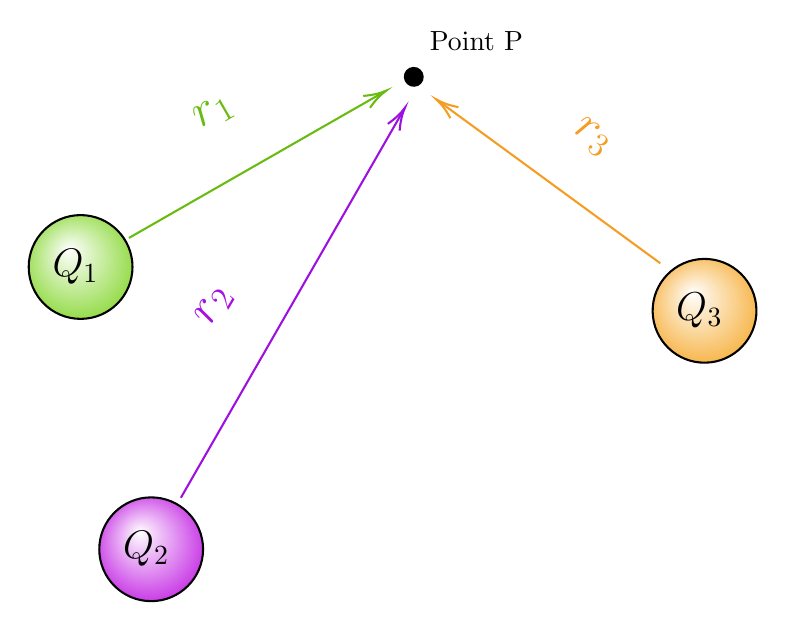
\begin{tikzpicture}[x=0.75pt,y=0.75pt,yscale=-1,xscale=1]
%uncomment if require: \path (0,300); %set diagram left start at 0, and has height of 300

%Shape: Circle [id:dp16269792186593102]
    \path  [shading=_brpskaxpq,_todkg7j90] (113,133) .. controls (113,119.19) and (124.19,108) .. (138,108) .. controls (151.81,108) and (163,119.19) .. (163,133) .. controls (163,146.81) and (151.81,158) .. (138,158) .. controls (124.19,158) and (113,146.81) .. (113,133) -- cycle ; % for fading
    \draw   (113,133) .. controls (113,119.19) and (124.19,108) .. (138,108) .. controls (151.81,108) and (163,119.19) .. (163,133) .. controls (163,146.81) and (151.81,158) .. (138,158) .. controls (124.19,158) and (113,146.81) .. (113,133) -- cycle ; % for border

%Straight Lines [id:da7734881847924964]
    \draw [color={rgb, 255:red, 106; green, 187; blue, 17 }  ,draw opacity=1 ]   (161.3,119) -- (283.56,48.99) ;
    \draw [shift={(285.3,48)}, rotate = 510.21] [color={rgb, 255:red, 106; green, 187; blue, 17 }  ,draw opacity=1 ][line width=0.75]    (10.93,-3.29) .. controls (6.95,-1.4) and (3.31,-0.3) .. (0,0) .. controls (3.31,0.3) and (6.95,1.4) .. (10.93,3.29)   ;
%Shape: Circle [id:dp3011729282954776]
    \draw  [fill={rgb, 255:red, 0; green, 0; blue, 0 }  ,fill opacity=1 ] (294.24,41.58) .. controls (294.11,39.22) and (295.92,37.22) .. (298.28,37.11) .. controls (300.64,37.01) and (302.67,38.84) .. (302.8,41.2) .. controls (302.93,43.56) and (301.13,45.56) .. (298.76,45.67) .. controls (296.4,45.77) and (294.38,43.94) .. (294.24,41.58) -- cycle ;
%Shape: Circle [id:dp023330508474848743]
    \path  [shading=_q7iq398zh,_8vthb5elb] (413.61,154.56) .. controls (413.36,140.75) and (424.35,129.36) .. (438.16,129.11) .. controls (451.96,128.86) and (463.36,139.85) .. (463.61,153.65) .. controls (463.86,167.46) and (452.87,178.85) .. (439.06,179.1) .. controls (425.26,179.35) and (413.87,168.36) .. (413.61,154.56) -- cycle ; % for fading
    \draw   (413.61,154.56) .. controls (413.36,140.75) and (424.35,129.36) .. (438.16,129.11) .. controls (451.96,128.86) and (463.36,139.85) .. (463.61,153.65) .. controls (463.86,167.46) and (452.87,178.85) .. (439.06,179.1) .. controls (425.26,179.35) and (413.87,168.36) .. (413.61,154.56) -- cycle ; % for border

%Straight Lines [id:da14629502647663206]
    \draw [color={rgb, 255:red, 245; green, 156; blue, 35 }  ,draw opacity=1 ][fill={rgb, 255:red, 245; green, 166; blue, 35 }  ,fill opacity=1 ]   (417.3,131.2) -- (310.91,53.38) ;
    \draw [shift={(309.3,52.2)}, rotate = 396.18] [color={rgb, 255:red, 245; green, 156; blue, 35 }  ,draw opacity=1 ][line width=0.75]    (10.93,-3.29) .. controls (6.95,-1.4) and (3.31,-0.3) .. (0,0) .. controls (3.31,0.3) and (6.95,1.4) .. (10.93,3.29)   ;
%Shape: Circle [id:dp3372508230198279]
    \path  [shading=_f2f473rbw,_5q0b6tgh9] (147,269) .. controls (147,255.19) and (158.19,244) .. (172,244) .. controls (185.81,244) and (197,255.19) .. (197,269) .. controls (197,282.81) and (185.81,294) .. (172,294) .. controls (158.19,294) and (147,282.81) .. (147,269) -- cycle ; % for fading
    \draw   (147,269) .. controls (147,255.19) and (158.19,244) .. (172,244) .. controls (185.81,244) and (197,255.19) .. (197,269) .. controls (197,282.81) and (185.81,294) .. (172,294) .. controls (158.19,294) and (147,282.81) .. (147,269) -- cycle ; % for border

%Straight Lines [id:da030140594007627808]
    \draw [color={rgb, 255:red, 156; green, 16; blue, 224 }  ,draw opacity=1 ]   (186.3,244.2) -- (293.3,57.93) ;
    \draw [shift={(294.3,56.2)}, rotate = 479.88] [color={rgb, 255:red, 156; green, 16; blue, 224 }  ,draw opacity=1 ][line width=0.75]    (10.93,-3.29) .. controls (6.95,-1.4) and (3.31,-0.3) .. (0,0) .. controls (3.31,0.3) and (6.95,1.4) .. (10.93,3.29)   ;

% Text Node
    \draw (123,123) node [anchor=north west][inner sep=0.75pt]  [font=\Large] [align=left] {$\displaystyle Q_{1}$};
% Text Node
    \draw (304.8,18.2) node [anchor=north west][inner sep=0.75pt]   [align=left] {Point P};
% Text Node
    \draw (188.99,57.01) node [anchor=north west][inner sep=0.75pt]  [font=\LARGE,color={rgb, 255:red, 106; green, 187; blue, 17 }  ,opacity=1 ,rotate=-330.07] [align=left] {$\displaystyle r_{1}$};
% Text Node
    \draw (423.34,144.38) node [anchor=north west][inner sep=0.75pt]  [font=\Large,rotate=-358.96] [align=left] {$\displaystyle Q_{3}$};
% Text Node
    \draw (380.52,57.74) node [anchor=north west][inner sep=0.75pt]  [font=\LARGE,color={rgb, 255:red, 245; green, 156; blue, 35 }  ,opacity=1 ,rotate=-35.56] [align=left] {$\displaystyle r_{3}$};
% Text Node
    \draw (157,259) node [anchor=north west][inner sep=0.75pt]  [font=\Large] [align=left] {$\displaystyle Q_{2}$};
% Text Node
    \draw (190.12,157.06) node [anchor=north west][inner sep=0.75pt]  [font=\LARGE,color={rgb, 255:red, 167; green, 16; blue, 224 }  ,opacity=1 ,rotate=-300.83] [align=left] {$\displaystyle r_{2}$};


\end{tikzpicture}